\documentclass{article}
\usepackage{amsfonts, amsmath, amssymb, amsthm, dsfont} % Math notations imported
\usepackage{enumitem}
\usepackage{graphicx}
\usepackage{setspace}
\usepackage{indentfirst}
\usepackage[margin=1in]{geometry}
\graphicspath{{./images/}} % Path to images

% \begin{figure}[htb!]
%      \centering
%      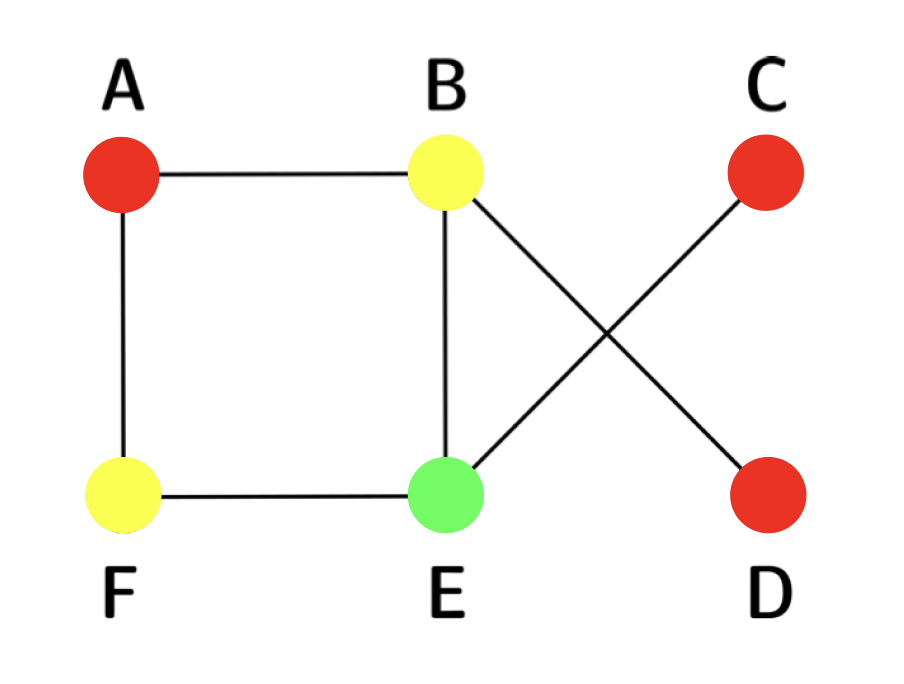
\includegraphics[scale=0.5]{coloring.png}
%      \caption{Coloring of the graph.}
% \end{figure}

% \begin{figure}[htb]
%     \qquad
%     \begin{minipage}{.4\textwidth}
%         \centering
%         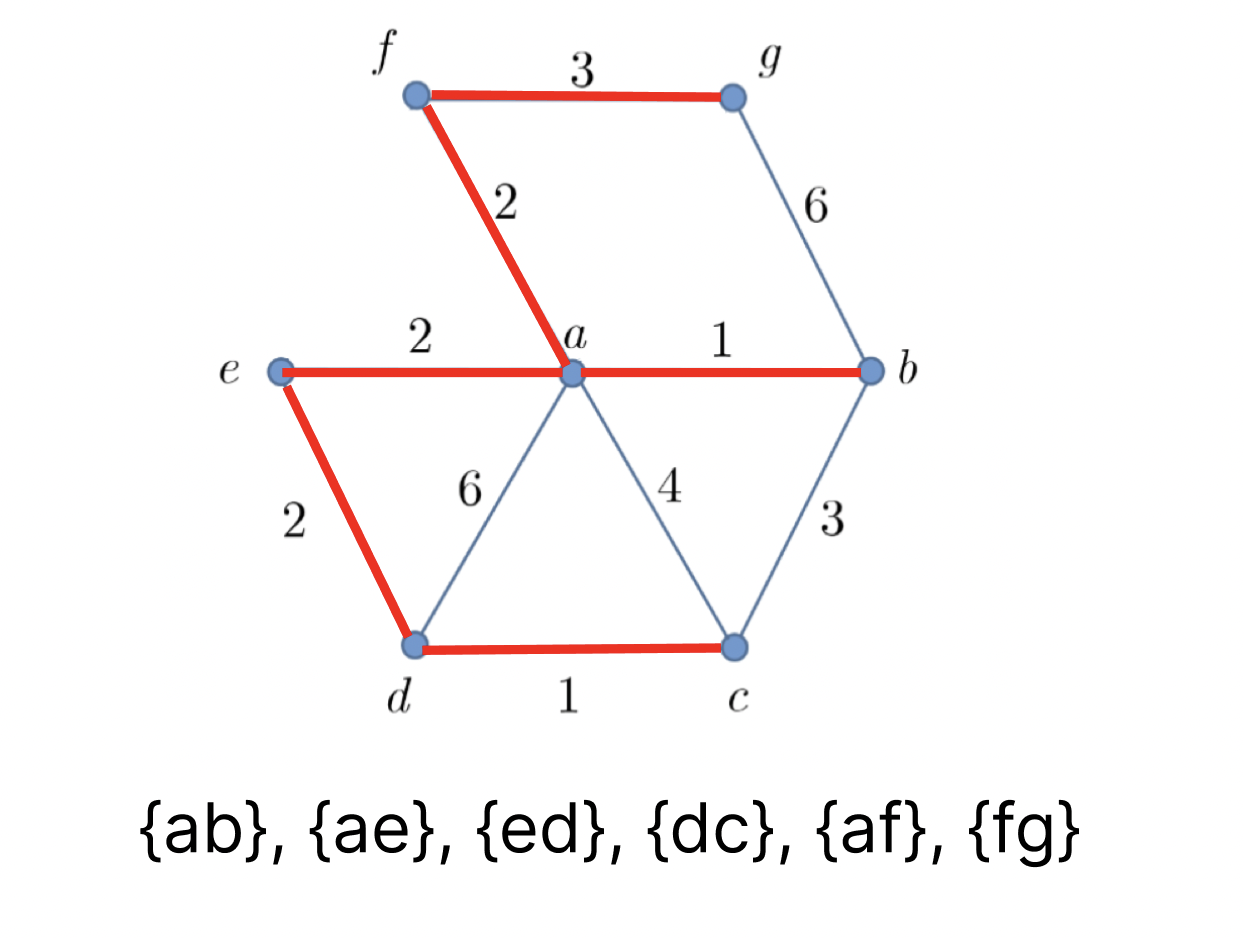
\includegraphics[scale=0.35]{prims.png}
%         \caption{}
%     \end{minipage}    
%     \qquad
%     \begin{minipage}{.4\textwidth}
%         \centering
%         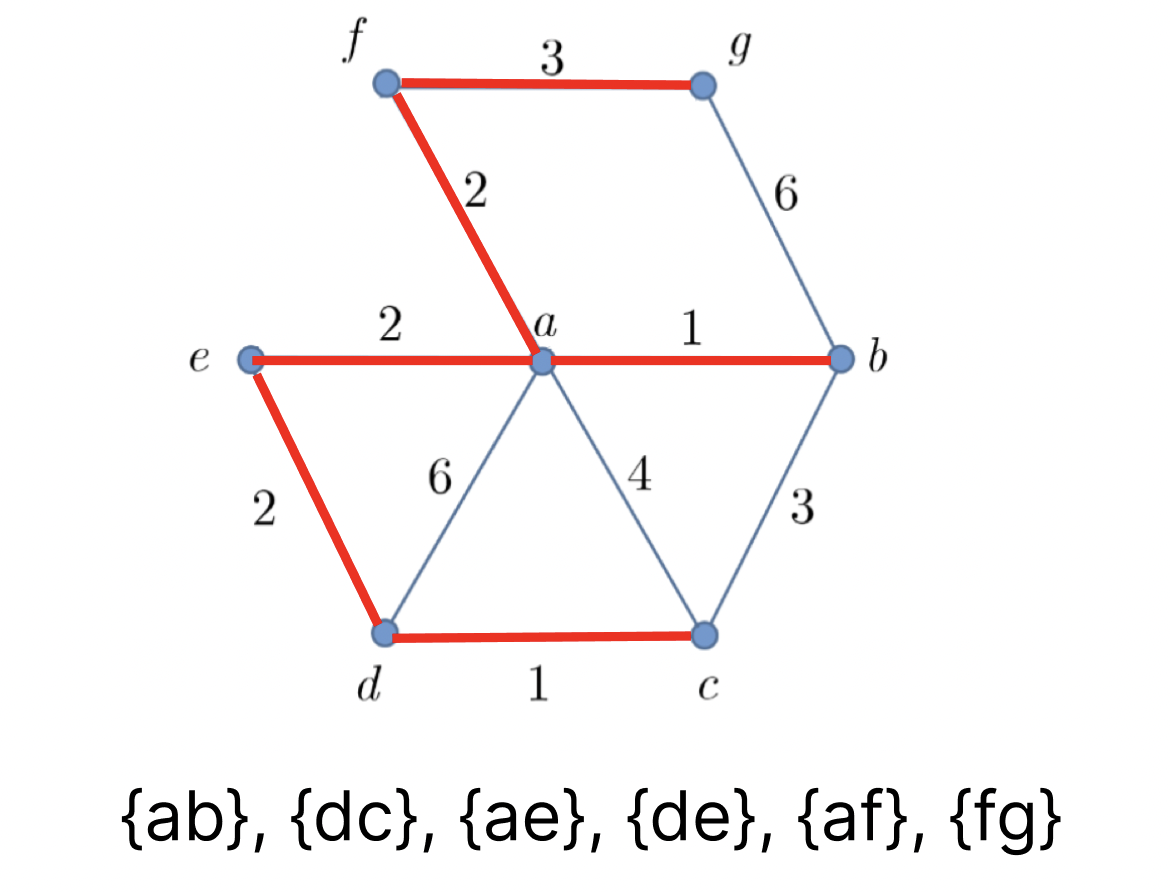
\includegraphics[scale=0.35]{kruskal.png}
%         \caption{}
%     \end{minipage}        
% \end{figure} 

\newtheorem{thm}{Theorem}
\newtheorem{proposition}[thm]{Proposition}
\newtheorem{corollary}[thm]{Corollary}
\newtheorem{lemma}[thm]{Lemma}

\newcommand*{\Var}{\ensuremath{\mathrm{Var}}}
\newcommand*{\Cov}{\ensuremath{\mathrm{Cov}}}
\newcommand*{\Corr}{\ensuremath{\mathrm{Corr}}}
\newcommand*{\Bias}{\ensuremath{\mathrm{Bias}}}
\newcommand*{\MSE}{\ensuremath{\mathrm{MSE}}}
\newcommand*{\range}{\ensuremath{\mathrm{range}}\,}
\newcommand*{\spann}{\ensuremath{\mathrm{span}}\,}
\newcommand*{\nul}{\ensuremath{\mathrm{null}}\,}
\newcommand*{\dom}{\ensuremath{\mathrm{dom}}\,}
\renewcommand*{\implies}{\ensuremath{\Longrightarrow}}
\renewcommand*{\impliedby}{\ensuremath{\Longleftarrow}}
\newcommand*{\Z}{\ensuremath{\mathbb{Z}}}
\newcommand*{\Q}{\ensuremath{\mathbb{Q}}}
\newcommand*{\R}{\ensuremath{\mathbb{R}}}
\newcommand*{\C}{\ensuremath{\mathbb{C}}}
\newcommand*{\N}{\ensuremath{\mathbb{N}}}
\newcommand*{\E}{\ensuremath{\mathds{E}}}
\renewcommand*{\P}{\ensuremath{\mathds{P}}}
\newcommand*{\p}{\ensuremath{\mathcal{P}}}

% title information
\title{Math 104 HW7}
\author{Neo Lee}
\date{27/10/2023}

\setstretch{1.15}
% main content
\begin{document} 

% placing title information; comment out if using fancyhdr
\maketitle 

\subsection*{Exercise 15.1}
Determine whether the following series converges:\qquad \textbf{(a)} $\sum \frac{(-1)^n}{n}$ 
\qquad \textbf{(b)} $\sum \frac{(-1)^nn!}{2^n}$.
\begin{proof}[Solution] \indent
    \begin{enumerate}[label=(\alph*)]
        \item 
        Consider $(a_n)=\frac{1}{n}$, then $a_n$ is an increasing sequence, and $\lim a_n=0$. By 
        Theorem 15.3, $\sum \frac{(-1)^n}{n}$ converges (Alternating Series).
        
        \item
        \begin{align*}
            \lim \left|\frac{a_{n+1}}{a_n}\right| & = \lim \left|\frac{(-1)^{n+1}(n+1)!}{2^{n+1}}\cdot
            \frac{2^n}{(-1)^nn!}\right| \\
            & = \lim \frac{n+1}{2} \\
            & = \infty.
        \end{align*}
        Hence, by Theorem 10.7, $\lim \inf \left|\frac{a_{n+1}}{a_n}\right| = 
        \lim \left|\frac{a_{n+1}}{a_n}\right| = \infty$. By Theorem 14.8, $\sum \frac{(-1)^nn!}{2^n}$
        containing non-zero terms diverges.
        diverges.
    \end{enumerate}
\end{proof}

\subsection*{Exercise 17.2}
Let $f(x)=4$ for $x\ge 0, f(x)=0$ for $x<0$, and $g(x)=x^2$ for all $x$. Thus $\dom(f)=\dom(g)=\R$.
\begin{enumerate}[label=(\alph*)]
    \item Determine the following functions: $f+g, fg, f\circ g, g\circ f$. Be sure to specify their 
    domain.
    \begin{proof}[Solution]\indent 
        \begin{enumerate}
            \item [($f+g$):] $$f+g:\R\to\R=\begin{cases}
                4+x^2 & x\ge 0 \\
                x^2 & x<0.
            \end{cases}$$
            \item [($fg$):] $$fg:\R\to\R=\begin{cases}
                4x^2 & x\ge 0 \\
                0 & x<0.
            \end{cases}$$
            \item [($f\circ g$):] $$f\circ g:\R\to\R=\begin{cases}
                4 & x\ge 0 \\
                0 & x<0.
            \end{cases}$$
            \item [($g\circ f$):] $$g\circ f:\R\to\R=\begin{cases}
                16 & x\ge 0 \\
                0 & x<0.
            \end{cases}$$
        \end{enumerate}
    \end{proof}

    \item Which of the functions $f,g,f+g,fg,f\circ g, g\circ f$ is continuous?
    \begin{proof}[Solution]\indent 
        \begin{enumerate}
            \item [($f$):]
            Not continuous. Consider $x_0=0$ and two sequences 
            $(s_n)=\frac{1}{n}, (t_n)=\frac{-1}{n}$. Then Then $\lim s_n=\lim t_n=0$, but
            $\lim f(s_n)=\lim 4 = 4\neq 0=\lim f(t_n) = \lim 0$.

            \item [($g$):]
            Continuous. Consider $x_0\in\R$. Then for any sequence $(s_n)\to x_0$, 
            $\lim g(s_n) = \lim s_n^2 = \lim s_n \cdot \lim s_n = x_0^2 = g(x_0)$.

            \item [($f+g$):] Not continuous. Consider $x_0=0$ and two sequences 
            $(s_n)=\frac{1}{n}$, $(t_n)=\frac{-1}{n}$. Then $\lim s_n=\lim t_n=0$, but
            $\lim (f+g)(s_n)=\lim 4 + \lim s_n \cdot \lim s_n = 4\neq 0=\lim (f+g)(t_n) = \lim t_n 
            \cdot \lim t_n$.

            \item [($fg$):] Continuous. Consider $(-\infty,0)$, $(0,\infty)$, and $0$. 
            
            For $x_0\in (-\infty,0)$, let $\delta = |x_0-0|$, then $|x-x_0|<\delta\implies f(x)=0=f(x_0)
            \implies |f(x)-f(x_0)|<\epsilon$ for $\epsilon>0$. 
            
            For $x_0\in (0,\infty)$, consider any sequence $(s_n)\to x_0$. Let $\epsilon = |x_0-0|$, 
            then $\exists N$ such that $|s_n-x_0|<\epsilon$ for $n>N$, which implies $s_n>0$ for 
            $n>N$. Then notice the limit of a sequence is independent of finite number of terms, 
            hence $\lim fg(s_n) = \lim fg(s_{n|n>N}) = \lim 4\cdot s_{n|n>N}\cdot s_{n|n>N} 
            = 4x_0^2 = fg(x_0)$.

            For $x_0 = 0$, take $\delta = \sqrt{\frac{\epsilon}{4}}$, then $|x-0|<\delta$ 
            $\implies |4x^2-0|=|f(x)-f(x_0)|<\epsilon$ for $x\ge 0$. If $x<0$, $f(x)=0$ and 
            obviously $|f(x)-f(x_0)|=0<\epsilon$.

            \item [($f\circ g$):] Not continuous. Consider $x_0=0$ and two sequences
            $(s_n)=\frac{1}{n}$, $(t_n)=\frac{-1}{n}$. Then $\lim s_n=\lim t_n=0$, but
            $\lim (f\circ g)(s_n)=\lim 4\neq 0=\lim (f\circ g)(t_n) = \lim 0$.

            \item [($g\circ f$):] Not continuous. Consider $x_0=0$ and two sequences
            $(s_n)=\frac{1}{n}$, $(t_n)=\frac{-1}{n}$. Then $\lim s_n=\lim t_n=0$, but
            $\lim (g\circ f)(s_n)=\lim 16\neq 0=\lim (g\circ f)(t_n) = \lim 0$.
        \end{enumerate}
        
    \end{proof}
\end{enumerate}
\subsection*{Exercise 17.13}
\begin{enumerate}[label=(\alph*)]
    \item \begin{proposition}
        Let $f(x)=1$ for $x\in\Q$ and $f(x)=0$ for $x\in\R\setminus\Q$. Then $f$ is discontinuous 
        at every $x\in\R$.
    \end{proposition}
    \begin{proof}\indent 
        \begin{enumerate}
            \item [\textbf{Case 1: }$x_0\notin\Q$.] Assume for the sake of contradiction that 
            $\exists \delta>0$ such that $|x-x_0|<\delta \implies |f(x)-f(x_0)|<1$. However, by 
            the density of $\Q$, $\exists x\in (x_0-\delta, x_0)$ such that $x$ is rational, 
            then $|f(x)-f(x_0)|=|1-0|=1\not< 1$, which is a contradiction.

            \item [\textbf{Case 2: }$x_0\in\Q$.] Assume for the sake of contradiction that
            $\exists \delta>0$ such that $|x-x_0|<\delta \implies |f(x)-f(x_0)|<1$. However, by
            the density of irrationals, $\exists x\in (x_0-\delta, x_0)$ such that $x$ is
            irrational, then $|f(x)-f(x_0)|=|0-1|=1\not< 1$, which is a contradiction.

            Note: density of irrationals was not covered in the book. But the proof idea is by 
            considering $\frac{a}{\sqrt{2}} < \frac{b}{\sqrt{2}}$, then there exists rational 
            $x$ in between. Multiplying the inequality by $\sqrt{2}$, we get $a <\sqrt{2}x<b$, 
            where $\sqrt{2}x$ is irrational.
        \end{enumerate}
    \end{proof}

    \item \begin{proposition}
        Let $h(x)=x$ for rational numbers $x$ and $h(x)=0$ for irrational numbers, then $h$ is
        continuous at $x=0$ and at no other point.
    \end{proposition}
    \begin{proof}\indent 
        \begin{enumerate}
            \item [$x_0=0$:] Let $\delta = \epsilon$, then if $x\in\Q$, $|x-x_0|=|x-0|<\delta\implies 
            |h(x)-h(x_0)|<\epsilon$. If $x\notin\Q$, $h(x)$ is always 0, hence 
            $|h(x)-h(x_0)|=0<\epsilon$.

            \item [$x_0\neq 0, x_0\in\Q$:] Let $\epsilon=|x_0|$. Assume for the sake of 
            contradiction that $\exists \delta>0$ such that $|x-x_0|<\delta\implies |h(x)-h(x_0)|
            <\epsilon$. However, by the density of irrationals, $\exists x\in (x_0-\delta, x_0)$
            such that $x$ is irrational, then $|h(x)-h(x_0)|=|0-x_0|=|x_0|=\epsilon\not<\epsilon$, 
            which is a contradiction.

            \item [$x_0\neq 0, x_0\notin\Q$:] Let $\epsilon=\frac{1}{2}|x_0|$. Assume for the sake 
            of contradiction that $\exists \delta>0$ such that $|x-x_0|<\delta\implies |h(x)-h(x_0)|
            <\epsilon$. However, by the density of $\Q$, $\exists x\in (x_0-\min\{\delta,\frac{1}{2}|x_0|\},
            x_0)$ such that $x$ is rational, then $|h(x)-h(x_0)|=|x-0|>\frac{1}{2}|x_0|
            \not <\epsilon$, which is a contradiction.
        \end{enumerate}
    \end{proof}
\end{enumerate}

\subsection*{Exercise 18.8}
\begin{proposition}
    Suppose $f$ is a real-valued continuous function on \R and $f(a)f(b)<0$ for some $a,b\in\R$, 
    then there exists $x\in (a,b)$ such that $f(x)=0$.
\end{proposition}
\begin{proof}
    Note that $f(a)\neq 0$ and $f(b)\neq 0$ and $f(a), f(b)$ cannot have the same sign. 
    Without loss of generality, assume $f(a)>0$ and $0>f(b)$. Then, by the Intermediate Value
    Theorem, $\exists x\in (a,b)$ such that $f(x)=0$.
\end{proof}

\end{document}
